% Source: Corsin Nick/Class Notes/Week 3.pdf, pp. 1--14
\chapter{Week 3 --- Compactness, Connectedness \& Cauchy--Schwarz}

% Transition: Claude Sonnet 5
This chapter finishes compactness (Heine--Borel, and why the property is useful in the first
place), introduces connectedness and path-connectedness, and then turns to the geometry of inner
product spaces: Cauchy--Schwarz, norms, and the Banach fixed point theorem. The exercise sheet is
at the end of the chapter, in \cref{sec:week03_solutions}.

\session{Monday}

\section{Compactness --- continued}
\label{sec:compactness_continued}
\continuedfrom{sec:compactness}

\begin{theorem}[Heine--Borel]
\label{thm:heine_borel}
A subset $K \subseteq \mathbb{R}^n$ equipped with the \textbf{standard metric} is
\textbf{compact} if and only if it is \newterm{closed} and \newterm{bounded}
(\germanterm{beschr\"ankt}).
\end{theorem}

\begin{ainote}
Neither Corsin nor this document proves \cref{thm:heine_borel}; it is proved in the lecture, and
the full argument is longer than anything else in these two chapters. It is worth knowing what
goes into it, though, since every ingredient has already appeared:
\begin{itemize}
  \item \textbf{($\Rightarrow$)} is short and general. A compact metric space is bounded and
    complete (\cref{lem:sequentially_compact_totally_bounded},
    \cref{ex:compact_finite_complete}), and a complete subset of the complete space
    $\mathbb{R}^n$ is closed (\cref{rem:complete_vs_closed}).
  \item \textbf{($\Leftarrow$)} is where the real content sits, and it is exactly
    \textbf{Bolzano--Weierstrass}: a bounded sequence in $\mathbb{R}^n$ has a convergent
    subsequence, obtained by bisecting a box $n$ times over, or by extracting coordinatewise
    (\cref{prop:Rn_coordinatewise_complete}) $n$ times in succession. Closedness then puts the
    limit back inside $K$, giving sequential compactness, which is compactness by
    \cref{thm:sequential_topological_compactness_equivalence}.
\end{itemize}
The reason the theorem is special to $\mathbb{R}^n$ with the standard metric is that both steps
use the completeness of $\mathbb{R}$ and the finiteness of the dimension.
\Cref{ex:heine_borel_fails} below shows how thoroughly it fails otherwise.
\end{ainote}

% Supplement: Sascha Brack/Class Notes/Week_02_Notes_Friday_Updated.pdf, p. 7
\begin{example}[Compactness via Heine-Borel and continuity]
\label{ex:compactness_heine_borel_examples}
Consider the following subsets and determine whether they are compact under the standard Euclidean metric:
\begin{enumerate}[label=\textbf{(\alph*)}]
  \item \textbf{Is $\mathbb{N} \subset \mathbb{R}$ compact?} No. While it is closed in $\mathbb{R}$, it is not bounded. By Heine-Borel, it cannot be compact.
  \item \textbf{Is $[0,1] \times [0,1] \subset \mathbb{R}^2$ complete?} Yes. The square $[0,1]^2$ is closed and bounded in $\mathbb{R}^2$, hence compact by Heine-Borel. As every compact metric space is complete (\cref{ex:compact_finite_complete}), it is complete.
  \item Let $f: \mathbb{R} \to \mathbb{R}^3, x \mapsto (\sin x, \cos x, 1)$. \textbf{Is $f([0,\pi/2])$ compact in $\mathbb{R}^3$?} Yes. We do not need to show this manually using sequences or open covers. Since the domain $[0,\pi/2]$ is compact in $\mathbb{R}$ (closed and bounded) and the function $f$ is continuous, its image $f([0,\pi/2])$ is compact in $\mathbb{R}^3$ (by \cref{item:continuity_preserves_compact}).
\end{enumerate}
\end{example}

% Supplement: Sascha Brack/Class Notes/Week_03_Notes_Monday.pdf, p. 3
\begin{exercise}[Topological properties of various subsets]
\label{ex:topological_properties_table}
Decide whether the following subsets are open, closed, compact, or complete (under the standard Euclidean metric):
\begin{enumerate}[label=\textbf{(\alph*)}]
  \item $[0,1] \subseteq \mathbb{R}$
  \item $\mathbb{Q} \subseteq \mathbb{R}$
  \item $B_1(0) \subseteq \mathbb{R}^3$
  \item $B_1(0) \cap B_1(1) \subseteq \mathbb{R}^2$
  \item $\{0\} \cup \{1/n \mid n \in \mathbb{N}_{\ge 1}\} \subseteq \mathbb{R}$
  \item $\bigcup_{n=1}^\infty B_{1/n}(n) \subseteq \mathbb{R}$
  \item $(-\infty, 1] \subseteq \mathbb{R}$
  \item $f([0,1])$ where $f : \mathbb{R} \to \mathbb{R}^n$ is continuous
  \item $f^{-1}([0,1])$ where $f : \mathbb{R}^n \to \mathbb{R}$ is continuous
  \item $f^{-1}((0,1))$ where $f : \mathbb{R}^n \to \mathbb{R}$ is continuous
  \item $S := \operatorname{span}\{(1,0,0)\transp, (3,1,0)\transp\} \subseteq \mathbb{R}^3$
  \item $\{x \in \mathbb{R}^3 \mid \exists s \in S \text{ s.t.\ } d(x, s) < 1\}$ for a subset $S \subseteq \mathbb{R}^3$
\end{enumerate}
\end{exercise}

\begin{exercisesolution}[Proof of \cref{ex:topological_properties_table}]
\begin{enumerate}[label=\textbf{(\alph*)}]
  \item $[0,1] \subseteq \mathbb{R}$: \textbf{Closed}, \textbf{compact}, \textbf{complete}. (Not open).
  \item $\mathbb{Q} \subseteq \mathbb{R}$: \textbf{None}. It is neither open nor closed, not bounded (so not compact), and not complete.
  \item $B_1(0) \subseteq \mathbb{R}^3$: \textbf{Open}.
  \item $B_1(0) \cap B_1(1) \subseteq \mathbb{R}^2$: \textbf{Open} (finite intersection of open sets).
  \item $\{0\} \cup \{1/n \mid n \in \mathbb{N}_{\ge 1}\} \subseteq \mathbb{R}$: \textbf{Closed}, \textbf{compact}, \textbf{complete} (bounded and contains its only limit point $0$).
  \item $\bigcup_{n=1}^\infty B_{1/n}(n) \subseteq \mathbb{R}$: \textbf{Open} (arbitrary union of open sets).
  \item $(-\infty, 1] \subseteq \mathbb{R}$: \textbf{Closed}, \textbf{complete}.
  \item $f([0,1])$: \textbf{Closed}, \textbf{compact}, \textbf{complete} (continuous image of a compact set).
  \item $f^{-1}([0,1])$: \textbf{Closed}, \textbf{complete} (continuous preimage of a closed set).
  \item $f^{-1}((0,1))$: \textbf{Open} (continuous preimage of an open set).
  \item $S := \operatorname{span}\{(1,0,0)\transp, (3,1,0)\transp\} \subseteq \mathbb{R}^3$: \textbf{Closed}, \textbf{complete} (it is a $2$-dimensional subspace, hence closed in $\mathbb{R}^3$).
  \item $\{x \in \mathbb{R}^3 \mid \exists s \in S \text{ s.t.\ } d(x, s) < 1\}$: \textbf{Open}. This set is equivalently written as $\{x \in \mathbb{R}^3 \mid d(x, S) < 1\}$ or $\bigcup_{s \in S} B_1(s)$, which is an arbitrary union of open balls.
\end{enumerate}
\end{exercisesolution}

This captures our intuition of a \qt{compact} set. We will briefly show that Heine--Borel is
\textbf{false} for $\mathbb{R}^n$ with an \textbf{arbitrary metric}.

\begin{exercise}[Heine--Borel fails for arbitrary metrics]
\label{ex:heine_borel_fails}
Let $(X,d)$ be a metric space.
\begin{enumerate}[label=\textbf{(\alph*)}]
  \item \textit{(Optional)} Show that $\tilde d(x,y) := \dfrac{d(x,y)}{1 + d(x,y)}$ is a metric on
    $X$.
  \item Show that, if $U \subseteq X$ is open with respect to $d$, then $U$ is open with respect
    to $\tilde d$.
  \item Show that, for $X = \mathbb{R}^n$, $d(x,y) = \dfrac{|x-y|}{1+|x-y|}$,
    $\mathbb{N} \subseteq X$ is closed and bounded but not compact.
\end{enumerate}
\end{exercise}

\begin{ainote}
Part \textbf{(c)} above sets $X = \mathbb{R}^n$ but then works with $\mathbb{N} \subseteq X$ and $|x-y|$,
which only parses for $n = 1$.
\end{ainote}

\begin{aiexample}[Open Cover of $(0,1)$ with No Finite Subcover]
% Generator: Gemini 3.6 Flash (Medium)
Consider the open interval $X = (0,1)$ under the standard Euclidean metric. The family of open sets
\[
U_n := \left(\frac{1}{n}, 1\right) \quad \text{for } n \in \mathbb{N}_{\ge 2}
\]
forms an open cover of $(0,1)$ because for any $x \in (0,1)$, there exists $n \in \mathbb{N}$ with $1/n < x$. However, any finite subcollection $\{U_{n_1}, \dots, U_{n_k}\}$ has a maximum index $N := \max\{n_1, \dots, n_k\}$, so its union is $U_N = (1/N, 1)$, which fails to cover points in $(0, 1/N]$. Thus $(0,1)$ is bounded but not compact.
\end{aiexample}

% Kept inline: solved directly in Corsin Nick/Class Notes/Week 3.pdf, pp. 1--2.
\begin{exercisesolution}[Proof of \cref{ex:heine_borel_fails}]
\textbf{(a)} Non-negativity, definiteness and symmetry are inherited directly from the
corresponding properties of $d$, since $t \mapsto \tfrac{t}{1+t}$ is non-negative on
$[0,\infty)$ and vanishes only at $t=0$.

\textit{Triangle inequality.} We want to show
\[
\frac{d(x,y)}{1+d(x,y)} \leq \frac{d(x,z)}{1+d(x,z)} + \frac{d(z,y)}{1+d(z,y)}.
\]
Denote $d(x,y) = d_1$, $d(x,z) = d_2$, $d(z,y) = d_3$ and multiply out:
\[
\begin{aligned}
&d_1(1+d_2)(1+d_3) \leq d_2(1+d_1)(1+d_3) + d_3(1+d_1)(1+d_2) \\
\iff\ & (d_1 + d_1d_2)(1+d_3) \leq (d_2 + d_2d_1)(1+d_3) + (d_3 + d_1d_3)(1+d_2) \\
\iff\ & d_1 + d_1d_3 + d_1d_2d_3 + d_1d_2 \leq d_2 + d_3d_2 + d_2d_1d_3 + d_2d_1 \\
& \qquad\qquad\qquad\qquad\qquad\quad + d_3 + d_3d_2 + d_1d_3 + d_1d_3d_2 \\
\iff\ & d_1 \leq d_2 + 2d_2d_3 + d_3 + d_1d_2d_3 \\
\Longleftarrow\ & 0 \leq 2d_2d_3 + d_1d_2d_3 \quad \text{together with } d_1 \leq d_2+d_3
  \text{ (the triangle inequality for } d\text{)}
\end{aligned}
\]
which is true by non-negativity.

\textbf{(b)} Let $U \subseteq X$ be open. Then, given $x \in U$, we find $r > 0$ such that
$B_r(x) := \{y \in X : d(x,y) < r\} \subseteq U$. Let $\varepsilon := \dfrac{r}{1+r}$. Then
$\tilde B_\varepsilon(x) \subseteq B_r(x) \subseteq U$, where
$\tilde B_\varepsilon(x) := \{y \in X : \tilde d(x,y) < \varepsilon\}$.

\textbf{(c)} Note that for all $x, y \in \mathbb{R}$, $\dfrac{|x-y|}{1+|x-y|} < 1$. So
$\mathbb{N} \subseteq B_1(0)$, thus it is \textbf{bounded} with respect to this metric. Also,
$\mathbb{N}$ is \textbf{closed}, as follows from \textbf{(b)}. But $x_n = n$ defines a sequence in
$\mathbb{N}$ with no convergent subsequence, thus $\mathbb{N}$ is \textbf{not compact}.
\end{exercisesolution}

\begin{ainote}
The cancellation in the derivation above originally contained a stray $d_2d_1d_2$ where the
expansion gives $d_2d_1d_3$; the cancelled terms and the conclusion $0 \leq 2d_2d_3 + d_1d_2d_3$
are unaffected. Re-derived cleanly above.
\end{ainote}

% Generator: Claude Opus 5 (Medium)
\begin{remark}[The moral: boundedness is not a topological property]
\label{rem:boundedness_not_topological}
It is worth saying out loud what \cref{ex:heine_borel_fails} has just demonstrated, because the
three parts are more striking together than separately.

Part \textbf{(b)} shows that $d$ and $\tilde d$ have the \emph{same open sets}. (Only one
direction is asked for, but the converse follows the same way: given
$\tilde B_\varepsilon(x)$, the choice $r := \tfrac{\varepsilon}{1-\varepsilon}$ gives
$B_r(x) \subseteq \tilde B_\varepsilon(x)$.) Two metrics with the same open sets have the same
convergent sequences, the same continuous functions, and --- crucially --- the same
\textbf{compact} sets, since compactness is defined purely by open covers
(\cref{def:compact_metric_space}).

Part \textbf{(c)} shows that they do \emph{not} have the same bounded sets. Indeed
$\tilde d < 1$ always, so under $\tilde d$ \emph{every} subset of \emph{every} metric space is
bounded --- the notion collapses entirely.

Putting those together: \textbf{compactness is topological, boundedness is not.} Boundedness is
a property of the chosen metric, not of the open sets it generates, so no theorem of the form
\qt{compact if and only if closed and bounded} can hold for a general metric. That is precisely why
\Cref{thm:heine_borel} carries the hypothesis \textbf{standard metric}, and it is not a
technicality to be skimmed --- it is the entire content of the hypothesis.

\begin{ainote}
The right general replacement is already in Week 2: compact if and only if complete \emph{and}
\newterm{totally bounded} (\cref{def:totally_bounded}, \cref{rem:compact_iff_complete_totally_bounded}).
Total boundedness is the notion boundedness was trying and failing to be, and $\mathbb{N}$ under
$\tilde d$ separates them cleanly: for $\varepsilon < \tfrac12$ the ball
$\tilde B_\varepsilon(n)$ contains no integer but $n$ itself, so no finite family of
$\varepsilon$-balls covers $\mathbb{N}$. Bounded, not totally bounded --- and that is exactly
the gap through which compactness escapes.
\end{ainote}
\end{remark}

\subsection{Why do we care about compactness?}

% Sonnet 5 (Medium): added \label on each item so these three facts (heavily cited by name in
% later chapters, e.g. the extreme value theorem) can be \cref-ed instead of just named in prose.
\begin{enumerate}[label=\textbf{(\alph*)}]
  \item \label{item:continuity_preserves_compact}
    \textbf{Preserved by continuous functions:} $X$, $Y$ metric spaces, $K \subseteq X$
    compact, $f : X \to Y$ continuous. Then $f(K) \subseteq Y$ is compact.
  \item \label{item:extreme_value_theorem}
    \textbf{Weierstrass theorem / Extreme value theorem:} $X$ metric space,
    $K \subseteq X$ compact, $f : K \to \mathbb{R}$ continuous. Then $f$ attains its maximum and
    minimum in $K$. In particular, $f$ is bounded --- proved as
    \Cref{lem:sequential_compactness_extreme_values} in Week 2.
  \item \label{item:uniform_continuity_compact}
    \textbf{Uniform continuity:} $X$, $Y$ metric spaces, $f : X \to Y$ continuous. If $X$ is
    compact, then $f$ is uniformly continuous (\cref{def:uniformly_continuous}) ---
    proved as \cref{prop:compact_implies_uniformly_continuous} in Week 2, via the Lebesgue number
    of the cover $\{f^{-1}(B_{\varepsilon/2}(y))\}_{y}$.
\end{enumerate}

% Sonnet 5 (Medium): illustrates item (b), the extreme value theorem.
\begin{center}
\begin{tikzpicture}[>=Latex, scale=1.2]
  \draw[->] (-0.3,0) -- (3.5,0) node[right] {$x$};
  \draw[->] (0,-0.3) -- (0,2.8) node[above] {$y$};

  \draw[green!60!black, thick] plot[smooth, tension=0.8] coordinates {(0.3,0.8) (0.9,2.3) (2.1,0.4) (3.0,1.8)};

  \draw (0.3,0.05) -- (0.3,-0.05) node[below] {$a$};
  \draw (0.9,0.05) -- (0.9,-0.05) node[below] {$c$};
  \draw (2.1,0.05) -- (2.1,-0.05) node[below] {$d$};
  \draw (3.0,0.05) -- (3.0,-0.05) node[below] {$b$};

  \draw[dashed, red!80!black] (0,2.3) node[left, font=\small] {$f(c)$} -- (0.9,2.3) -- (0.9,0);
  \fill[red!80!black] (0.9,2.3) circle (2pt);

  \draw[dashed, blue!80!black] (0,0.4) node[left, font=\small] {$f(d)$} -- (2.1,0.4) -- (2.1,0);
  \fill[blue!80!black] (2.1,0.4) circle (2pt);

  \node[below, font=\small, align=center] at (1.7,-0.55)
    {\textbf{(b)} on the compact $K=[a,b]$, $f$ attains its maximum at $c$ and its minimum at $d$};
\end{tikzpicture}
\end{center}

Both extrema are attained \emph{inside} $K$ --- that is the content of \textbf{(b)}, and it is
exactly what fails on a non-compact domain: on the open interval $(a,b)$ the same $f$ may
approach a supremum it never reaches.

% Quelle: Diego Torres Tejeda/Notes - 02.03 - Diego Torres Tejeda.pdf, pp. 8--10
\begin{remark}[What compactness and connectedness are \emph{for}: local to global]
\label{rem:local_to_global}
The three facts above look like a list of unrelated services compactness happens to provide.
Diego Torres Tejeda's notes give the idea that unifies them, and it is worth having early
because it also explains why connectedness sits in the same chapter.

\textbf{Local-to-global arguments} are a recurring theme across mathematics. It is often easy to
check a property \emph{locally} --- on some ball $B_\varepsilon(x)$ around each point --- and
what one actually wants is the property \emph{globally}, on all of $X$. Compactness and
connectedness are the two hypotheses that license that jump. Schematically, a local-to-global
statement reads:
\begin{quote}
\itshape
If for every $x \in X$ there is $\varepsilon>0$ such that $B_\varepsilon(x)$ has property $P$,
then $X$ has property $P$.
\end{quote}
Each of the two hypotheses powers its own version, and the proofs are three lines each.

\textbf{Connectedness turns \qt{locally constant} into \qt{constant}.} Let $(X,d)$ be connected
and $f : X \to \mathbb{R}$ locally constant. Every level set $f^{-1}(a)$ is then open. Fix
$a \in f(X)$ and split
\[X = \underbrace{f^{-1}(a)}_{=:U} \ \sqcup \underbrace{\bigcup_{b \neq a}f^{-1}(b)}_{=:V},\]
a disjoint union of two open sets. Since $U \neq \emptyset$, connectedness forces $V=\emptyset$,
i.e.\ $f \equiv a$.

\textbf{Compactness turns \qt{locally bounded} into \qt{bounded}.} Let $X$ be compact and
suppose each $x$ has an open $U_x \ni x$ on which $f$ is bounded. The $\{U_x\}_{x\in X}$ cover
$X$, so finitely many suffice, say $U_1,\dots,U_n$, and then
\[\sup_{x \in X}|f(x)| \;=\; \max_{1\leq i\leq n}\ \sup_{x \in U_i}|f(x)| \;<\; \infty,\]
because a \emph{maximum of finitely many} finite numbers is finite. Taking $f$ continuous ---
which is locally bounded, since $|f|<|f(x)|+1$ near each $x$ --- recovers the boundedness half
of \cref{item:extreme_value_theorem}.

Read this way the two proofs are the same proof twice, with different notions of \qt{finitely
many}: connectedness says a partition into two open pieces must be trivial, compactness says a
cover can be taken finite. Both convert local information into global. Every application in
\Cref{item:continuity_preserves_compact,item:extreme_value_theorem,item:uniform_continuity_compact}
is an instance --- uniform continuity most visibly, where the whole difficulty is that the
$\delta$ from continuity is local and one needs a single global one
(\cref{rem:continuity_vs_uniform_continuity}).
\end{remark}

\begin{ainote}
The exercise below overlaps heavily with \cref{ex:topological_properties_table} above --- both
are Sascha Brack's, from two different files (his Week 2 Friday and Week 3 Monday notes), and
he evidently reused the self-test. Both are kept, because deciding that one of them is redundant
is a judgement about his notes rather than about this transcription, and the second version does
add three things: the explicit \textbf{?} answers where the data is insufficient, the trap in
the final item (two \emph{parallel} spanning vectors), and the four-column table format of the
solution, which is where the lesson actually lands. Read
\cref{ex:topological_properties_table} as the warm-up and this one as the real test.
\end{ainote}

% Supplement: Sascha Brack/Class Notes/Week_02_Notes_Friday_Updated.pdf, p. 8
\begin{exercise}[Classify these sets]
\label{ex:classification_table}
Sascha Brack sets this as a self-test at the end of his compactness lecture, and it is the
fastest way to find out whether the four notions have actually separated in your head. For each
subset of $\mathbb{R}^n$ (standard metric), decide whether it is \textbf{open}, \textbf{closed},
\textbf{compact}, \textbf{complete}. Throughout, $f$ denotes a continuous function and
\textbf{?} means \qt{not decidable from the information given}.
\begin{enumerate}[label=\textbf{\arabic*.}]
  \item $[0,1] \subseteq \mathbb{R}$
  \item $\mathbb{Q} \subseteq \mathbb{R}$
  \item $B_1(0) \subseteq \mathbb{R}^3$
  \item $\left\{\tfrac1n : n \geq 1\right\} \subseteq \mathbb{R}$, and separately
    $\{0\} \cup \left\{\tfrac1n : n \geq 1\right\}$
  \item $\bigcup_{n\geq1}B_{1/n}(n) \subseteq \mathbb{R}$
  \item $(-\infty,1] \subseteq \mathbb{R}$
  \item $f([0,1])$, \quad $f^{-1}([0,1])$, \quad $f^{-1}\big((0,1)\big)$
  \item $S := \operatorname{span}\!\left\{\begin{pmatrix}1\\0\end{pmatrix},
    \begin{pmatrix}3\\0\end{pmatrix}\right\} \subseteq \mathbb{R}^2$
\end{enumerate}
\end{exercise}

% Quelle: Diego Torres Tejeda/Notes - 16.03 - Diego Torres Tejeda.pdf, p. 1 -- Sonnet 5 (Medium)
\begin{remark}[What continuous maps do and do not preserve]
Diego's exercise-class notes collect \cref{item:continuity_preserves_compact} and the analogous
fact for connectedness (\cref{thm:continuity_preserves_connected}) into one table, together with
the dual statement for preimages, and a caution worth stating explicitly:
\begin{center}
\begin{tabular}{lll}
& \textbf{Preserved by $f^{-1}$} & \textbf{Preserved by $f$} \\
\hline
open & yes (\cref{def:continuous}) & not in general \\
closed & yes & not in general \\
compact & not in general & yes (\cref{item:continuity_preserves_compact}) \\
connected & not in general & yes (\cref{thm:continuity_preserves_connected}) \\
\end{tabular}
\end{center}
\textbf{Caution:} completeness and boundedness are \emph{not} topological properties, so they
are not preserved by continuous maps or their inverses in general --- e.g.\ $\tan :
(-\tfrac\pi2,\tfrac\pi2) \to \mathbb{R}$ is a continuous bijection from a bounded set onto an
unbounded one.
\end{remark}

% Quelle: Linus Lüchinger/Slides/Slides-03-02.pdf, pp. 10--13 -- Sonnet 5 (Medium)
\begin{ainote}
Corsin never formally introduces Lipschitz continuity, even though a Lipschitz
constant is already used informally for contraction mappings
(\cref{def:contraction_mapping}, below). Lüchinger's exercise slides motivate and name it as a
strictly stronger condition than uniform continuity, and give a quick self-test; both are
reproduced here (reformulated), since they fill a genuine gap.
\end{ainote}

\begin{definition}[Lipschitz continuity]
\label{def:lipschitz_continuous}
Let $(X,d_X)$, $(Y,d_Y)$ be metric spaces. A function $f : X \to Y$ is \newterm{Lipschitz
continuous} (\germanterm{Lipschitz-stetig}) if there exists $L \geq 0$, a \newterm{Lipschitz
constant} for $f$, such that
\[d_Y(f(x),f(x')) \leq L\cdot d_X(x,x') \quad \text{for all } x,x' \in X.\]
\end{definition}

\begin{remark}[Hierarchy of continuity notions]
\label{rem:continuity_hierarchy}
Lipschitz continuity is stronger than uniform continuity
(\cref{def:uniformly_continuous}), which in turn is stronger than continuity
(\cref{def:continuous}). For the first implication, assume $L > 0$ (for $L = 0$ the function is
constant and there is nothing to prove); then $\delta := \varepsilon/L$ satisfies the definition
of uniform continuity, since
\[d_X(x,x') < \frac{\varepsilon}{L} \quad \text{gives} \quad d_Y(f(x),f(x')) \leq L\,d_X(x,x') < \varepsilon\]
for \emph{every} pair $x,x'$ --- the same $\delta$ at every point, which is exactly what
uniform continuity asks for. The second implication is immediate: a $\delta$ that works at all
points in particular works at each one.

Both converses fail. Every continuously differentiable function on a compact \emph{interval} is
Lipschitz continuous, with $L := \sup|f'|$ by the mean value theorem --- the interval matters,
since the mean value theorem needs the segment between the two points to lie in the domain ---
but $f(x) := \sqrt{x}$ on
$[0,\infty)$ is uniformly continuous and \emph{not} Lipschitz: a Lipschitz constant would force
$\delta$ to shrink only linearly in $\varepsilon$, whereas here
$|\sqrt{x}-\sqrt{x'}| < \varepsilon$ near $0$ already requires $\delta$ of order
$\varepsilon^2$. The reason is visible in the graph --- the tangent at $0$ is vertical, so no
finite slope $L$ can dominate it.
\end{remark}

% Sonnet 5 (Medium)
\begin{center}
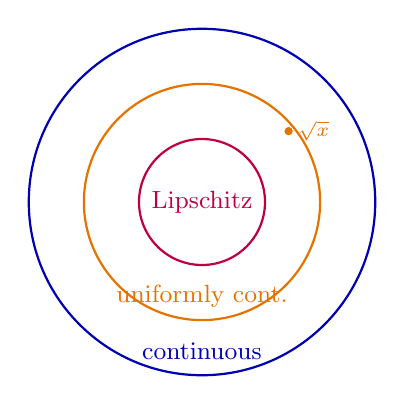
\begin{tikzpicture}[scale=1.0]
  \draw[blue!70!black, thick] (0,0) circle (2.2);
  \node[blue!70!black, font=\small] at (0,-1.9) {continuous};
  \draw[orange!90!black, thick] (0,0) circle (1.5);
  \node[orange!90!black, font=\small] at (0,-1.2) {uniformly cont.};
  \draw[purple, thick] (0,0) circle (0.8);
  \node[purple, font=\small] at (0,0) {Lipschitz};
  \fill[orange!90!black] (1.1,0.9) circle (1.5pt) node[right, font=\scriptsize] {$\sqrt{x}$};
\end{tikzpicture}
\end{center}

\begin{aiexercise}[Classifying continuity]
\label{ex:ai_continuity_classification}
% Generator: Claude Sonnet 5 (Medium), after Linus Lüchinger/Slides/Slides-03-02.pdf, p. 13
For each of the following functions, determine whether it is continuous, uniformly continuous,
and/or Lipschitz continuous on the given domain:
\begin{center}
\begin{tabular}{ll}
\textbf{Function} & \textbf{Domain} \\
\hline
$\sqrt{x}$ & $[0,\infty)$ \\
$1/x$ & $(0,1)$ \\
$\sgn(x)$ & $(-1,1)$ \\
$|x|^{3/2}$ & $(-1,1)$
\end{tabular}
\end{center}
\end{aiexercise}

% Sonnet 5 (Medium)
Compactness told us when a space has \qt{enough finiteness} to guarantee extrema and uniform
behaviour. We now turn to a completely different, qualitative kind of structure: whether a space
can be split into separate pieces at all.

\section{Connectedness}
\label{sec:connectedness}

\begin{definition}[Connected and disconnected metric spaces]
\label{def:connectedness}
A metric space $(X,d)$ is \newterm{disconnected} (\germanterm{unzusammenh\"angend}) if there
exist $U_1, U_2 \subseteq X$ subsets which are
\begin{enumerate}[label=\textbf{(\alph*)}]
  \item \textbf{open},
  \item \textbf{non-empty}, $U_1 \neq \emptyset \neq U_2$,
  \item \textbf{disjoint}, $U_1 \cap U_2 = \emptyset$,
\end{enumerate}
such that $X = U_1 \cup U_2$. Similarly, for a subset $A \subseteq X$, it is disconnected if it is
disconnected as a metric space with the induced metric $d|_{A \times A}$. \newterm{Connected}
(\germanterm{zusammenh\"angend}) is the negation of disconnected.
\end{definition}

Typically, proving that a set or metric space is connected is done \textbf{by contradiction},
which is why one should remember the definition of \textit{disconnected}. Intuitively, connected
means: \qt{the space cannot be separated by open sets.}

\begin{center}
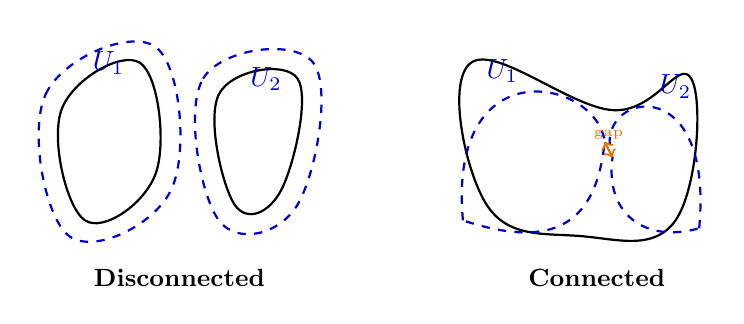
\begin{tikzpicture}[scale=1.0]
  % Left panel: Disconnected
  \begin{scope}[shift={(0,0)}]
    \draw[thick] plot[smooth cycle, tension=0.7] coordinates {(-1.5,-0.8) (-1.8,0.6) (-0.8,1.2) (-0.6,-0.2)};
    \draw[thick] plot[smooth cycle, tension=0.7] coordinates {(0.4,-0.6) (0.2,0.8) (1.2,1.0) (1.0,-0.4)};

    \draw[blue!80!black, thick, dashed] plot[smooth cycle, tension=0.7] coordinates {(-1.7,-1.0) (-2.0,0.8) (-0.6,1.4) (-0.4,-0.4)};
    \node[blue!80!black] at (-1.2,1.2) {$U_1$};

    \draw[blue!80!black, thick, dashed] plot[smooth cycle, tension=0.7] coordinates {(0.2,-0.8) (0.0,1.0) (1.4,1.2) (1.2,-0.6)};
    \node[blue!80!black] at (0.8,1.0) {$U_2$};

    \node[below, font=\small] at (-0.3,-1.3) {\textbf{Disconnected}};
  \end{scope}

  % Right panel: Connected
  \begin{scope}[shift={(5.0,0)}]
    \draw[thick] plot[smooth cycle, tension=0.7] coordinates {(-1.4,-0.6) (-1.6,1.2) (0.2,0.6) (1.2,1.0) (1.0,-0.8) (-0.2,-1.0)};

    \draw[blue!80!black, thick, dashed] (-1.7,-0.8).. controls (-1.9,1.4) and (0.0,1.0).. (0.1,0.2).. controls (0.0,-0.8) and (-0.5,-1.2).. (-1.7,-0.8);
    \node[blue!80!black] at (-1.2,1.1) {$U_1$};

    \draw[blue!80!black, thick, dashed] (1.3,-0.9).. controls (1.5,1.2) and (-0.1,0.8).. (0.2,0.0).. controls (0.1,-0.7) and (0.6,-1.1).. (1.3,-0.9);
    \node[blue!80!black] at (1.0,0.9) {$U_2$};

    \draw[orange!90!black, <->, thick] (0.1,0.2) -- node[above, font=\tiny] {gap} (0.2,0.0);

    \node[below, font=\small] at (0,-1.3) {\textbf{Connected}};
  \end{scope}
\end{tikzpicture}
\end{center}

% Generator: Claude Opus 5 (High) --- the base case of connectedness, used three times in this
% chapter (path-connectedness, the topologist's sine curve, the intermediate value theorem)
% but stated nowhere in the source notes.
\begin{proposition}[Intervals are connected]
\label{prop:intervals_connected}
Every interval $I \subseteq \mathbb{R}$ --- open, closed, half-open, bounded or not --- is
connected (\cref{def:connectedness}). Conversely, a connected subset of $\mathbb{R}$ is an
interval.
\end{proposition}

\begin{proof}
Suppose $I = U_1 \sqcup U_2$ with $U_1, U_2$ open in $I$, disjoint and both non-empty. Pick
$a \in U_1$ and $b \in U_2$; without loss of generality $a<b$, and $[a,b] \subseteq I$ because
$I$ is an interval. Set
\[c := \sup\{\,t \in [a,b] \ :\ [a,t] \subseteq U_1\,\},\]
which is well defined since $a$ belongs to the set. Now $c \in [a,b] \subseteq I$, so $c$ lies
in $U_1$ or in $U_2$, and both lead to a contradiction:
\begin{itemize}
  \item If $c \in U_1$, openness gives $\varepsilon>0$ with $(c-\varepsilon,c+\varepsilon)\cap I
    \subseteq U_1$; together with $[a,c) \subseteq U_1$ this yields $[a,t] \subseteq U_1$ for
    some $t>c$ unless $c=b$ --- contradicting either the supremum or $b \in U_2$.
  \item If $c \in U_2$, openness gives $\varepsilon>0$ with $(c-\varepsilon,c] \cap I \subseteq
    U_2$. But $c>a$ (as $a \in U_1$ is open in $I$), so by definition of the supremum there is
    $t \in (c-\varepsilon,c]$ with $[a,t] \subseteq U_1$ --- contradicting disjointness.
\end{itemize}
So no such splitting exists, and $I$ is connected. For the converse, a set $A \subseteq
\mathbb{R}$ that is not an interval admits $a<c<b$ with $a,b \in A$ and $c \notin A$; then
$A \cap (-\infty,c)$ and $A \cap (c,\infty)$ disconnect it.
\end{proof}

\begin{remark}[Why this is the only example one ever needs]
\label{rem:intervals_are_the_base_case}
Every connectedness proof in this chapter reduces to \cref{prop:intervals_connected}: a path is
a continuous image of $[0,1]$ (\cref{def:path}), so path-connected sets are connected
(\cref{lem:path_connected_implies_connected}) purely because the \emph{interval} is; and the
intermediate value theorem, invoked in the topologist's sine curve below, is
\cref{thm:continuity_preserves_connected} applied to an interval, since the connected subsets of
$\mathbb{R}$ are exactly the intervals. In other words, the single fact that $\mathbb{R}$ has no
gaps --- the completeness axiom, which is what powers the supremum above --- is the source of
all of it.
\end{remark}

\begin{aiexample}[Disconnectedness of Rational Numbers]
% Generator: Gemini 3.6 Flash (Medium)
The set of rational numbers $\mathbb{Q} \subset \mathbb{R}$ equipped with the subspace topology is disconnected. To see this, define
\[
U := \mathbb{Q} \cap (-\infty, \sqrt{2}) \quad \text{and} \quad V := \mathbb{Q} \cap (\sqrt{2}, \infty).
\]
Since $\sqrt{2} \notin \mathbb{Q}$, we have $U \cup V = \mathbb{Q}$ and $U \cap V = \emptyset$. Both $U$ and $V$ are non-empty and open in the subspace topology of $\mathbb{Q}$ (as intersections of $\mathbb{Q}$ with open intervals in $\mathbb{R}$). Hence $U$ and $V$ form a separation of $\mathbb{Q}$.
\end{aiexample}

% Supplement: Sascha Brack/Class Notes/Week_02_Notes_Friday_Updated.pdf, p. 9
\begin{example}[A disconnected set in $\mathbb{R}^2$]
Let $X := ([0,1] \times [0,1]) \cup ([2,3] \times \{1\}) \subseteq \mathbb{R}^2$. Is $X$ connected?
No. Let $U := \{(x,y) \in X \mid x < 1.5\}$ and $V := \{(x,y) \in X \mid x > 1.5\}$. We can write these as $U = X \cap \{(x,y) \in \mathbb{R}^2 \mid x < 1.5\}$ and $V = X \cap \{(x,y) \in \mathbb{R}^2 \mid x > 1.5\}$. Both $U$ and $V$ are open in the subspace topology of $X$ because they are intersections of $X$ with open half-planes in $\mathbb{R}^2$. Furthermore, $X = U \cup V$, and $U, V$ are disjoint and non-empty. Thus, $X$ is disconnected.
\end{example}

\begin{theorem}[Continuous functions preserve connectedness]
\label{thm:continuity_preserves_connected}
Let $X$, $Y$ be metric spaces, $f : X \to Y$ continuous. If $A \subseteq X$ is connected, then
$f(A)$ is connected.
\end{theorem}

% Generator: Claude Opus 5 (High) --- stated without proof in the source; the argument is three
% lines and is the exact dual of \cref{item:continuity_preserves_compact}.
\begin{proof}
We may assume $A = X$, replacing $X$ by $A$ with the induced metric and $Y$ by $f(A)$. Suppose
$f(X)$ were disconnected, say $f(X) = V_1 \sqcup V_2$ with $V_1,V_2$ open in $f(X)$, disjoint
and non-empty. Then $U_i := f^{-1}(V_i)$ is open by \cref{def:continuous}\textbf{(c)},
non-empty because $V_i$ meets the image, and $U_1 \cap U_2 = \emptyset$ with
$U_1 \cup U_2 = X$ because the $V_i$ partition $f(X)$. So $U_1,U_2$ disconnect $X$, contrary to
hypothesis.
\end{proof}

\begin{corollary}[Intermediate value theorem]
\label{cor:intermediate_value_theorem}
Let $f : [a,b] \to \mathbb{R}$ be continuous. Then $f$ attains every value between $f(a)$ and
$f(b)$.
\end{corollary}

\begin{proof}
By \cref{prop:intervals_connected}, $[a,b]$ is connected, so $f([a,b])$ is connected by
\cref{thm:continuity_preserves_connected}, hence is an interval (\cref{prop:intervals_connected}
again). An interval containing $f(a)$ and $f(b)$ contains everything between them.
\end{proof}

\begin{ainote}
The intermediate value theorem is a result from \emph{Analysis I}, but it is worth re-deriving
it here in one line: it is the first place where connectedness earns its keep, and the proof
makes visible that the theorem is really a statement about $\mathbb{R}$ having no gaps rather
than about $f$. It is used in the topologist's sine curve
(\cpageref{ex:topologists_sine_curve}) below.
\end{ainote}

% Supplement: Sascha Brack/Class Notes/Week_03_Notes_Monday.pdf, p. 4
\begin{corollary}[Linear maps preserve the unit cube]
\label{cor:linear_maps_unit_cube}
Given the $n$-dimensional unit cube $[0,1]^n \subset \mathbb{R}^n$, any linear map $L : \mathbb{R}^n \to \mathbb{R}^n$ maps $[0,1]^n$ to an $n$-dimensional parallelepiped. Since linear maps in Euclidean space are continuous, the image $L([0,1]^n)$ is connected. Furthermore, since $[0,1]^n$ is compact, $L([0,1]^n)$ is also compact.
\end{corollary}

\begin{exercise}[Properties of connectedness]
\label{ex:connectedness_tf}
Are the following true or false?
\begin{enumerate}[label=\textbf{(\alph*)}]
  \item The union of connected subsets with a common point is connected.
  \item The intersection of connected subsets is connected.
  \item The \newterm{closure} (\germanterm{Abschluss}, \cref{def:interior_closure_boundary}) of a
    connected subset is connected.
\end{enumerate}
\end{exercise}

% Kept inline: solved directly in Corsin Nick/Class Notes/Week 3.pdf, pp. 5--6.
\begin{exercisesolution}[Proof of \cref{ex:connectedness_tf}]
\textbf{(a) True.} \textit{Proof.} Let $X$ be a metric space, $V_1, V_2 \subseteq X$ connected,
and $x_0 \in V_1 \cap V_2$. Suppose $V_1 \cup V_2 \subseteq U_1 \cup U_2$ with
$U_1, U_2 \subseteq X$ open and disjoint. Assume without loss of generality $x_0 \in U_1$. Then
$U_1 \cap V_1 \neq \emptyset$ and $U_1 \cap V_2 \neq \emptyset$. So, since $V_1, V_2$ are
connected, $V_1 \cap U_2 = V_2 \cap U_2 = \emptyset$. Therefore
$(V_1 \cup V_2) \cap U_2 = \emptyset$ and $V_1 \cup V_2$ is connected.

\textbf{(b) False.} \textit{Counterexample:}
\[
X = \mathbb{R}^2, \quad U = [-1,1] \times \{0\}, \quad V = S^1 = \{x \in \mathbb{R}^2 : \|x\| = 1\},
\]
\[
U \cap V = \{(-1,0), (1,0)\}.
\]

\textbf{(c) True.} Suppose $X$ is a metric space, $A \subseteq X$ a subset with closure
$\overline{A}$. Suppose $U_1, U_2 \subseteq X$ are disjoint open sets covering $\overline{A}$, and
assume without loss of generality $\overline{A} \cap U_1 \neq \emptyset$. Then, since $U_1$ is
open, $A \cap U_1 \neq \emptyset$. By connectedness of $A$, $U_2 \cap A = \emptyset$, and since
$U_2$ is open, also $U_2 \cap \overline{A} = \emptyset$.
\end{exercisesolution}

\begin{ainote}
Corsin writes $\|x\| = R^2$ in the definition of $S^1$ above; it must be $\|x\| = 1$, as the
stated intersection $\{(\pm 1, 0)\}$ confirms. Corrected here.
\end{ainote}

\begin{center}
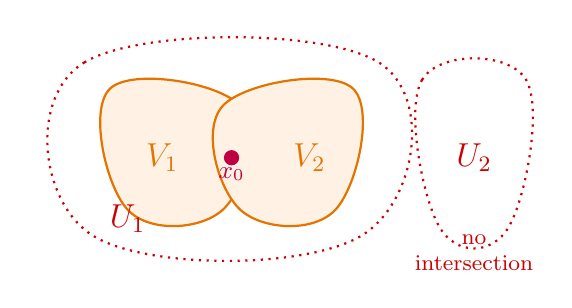
\begin{tikzpicture}[scale=1.1]
  \draw[orange!90!black, thick, fill=orange!10] plot[smooth cycle, tension=0.7] coordinates {(-1.6,-0.6) (-1.8,0.8) (-0.3,0.6) (-0.5,-0.6)};
  \node[orange!90!black, font=\large] at (-1.2,0) {$V_1$};

  \draw[orange!90!black, thick, fill=orange!10] plot[smooth cycle, tension=0.7] coordinates {(-0.3,-0.6) (-0.5,0.6) (1.0,0.8) (0.8,-0.6)};
  \node[orange!90!black, font=\large] at (0.5,0) {$V_2$};

  \fill[purple] (-0.4,0) circle (2.5pt) node[below, font=\small] {$x_0$};

  \draw[red!80!black, thick, dotted] plot[smooth cycle, tension=0.7] coordinates {(-2.0,-0.9) (-2.1,1.1) (1.3,1.1) (1.1,-0.9)};
  \node[red!80!black, font=\large] at (-1.6,-0.7) {$U_1$};

  \draw[red!80!black, thick, dotted] plot[smooth cycle, tension=0.7] coordinates {(2.0,-0.8) (1.8,0.9) (3.0,0.9) (2.8,-0.8)};
  \node[red!80!black, font=\large] at (2.4,0) {$U_2$};
  \node[red!80!black, font=\footnotesize, align=center] at (2.4,-1.1) {no\\intersection};
\end{tikzpicture}
\end{center}

\begin{center}
\begin{tikzpicture}[>=Latex, scale=1.3]
  \draw[->] (-1.6,0) -- (1.6,0) node[right] {$x$};
  \draw[->] (0,-1.6) -- (0,1.6) node[above] {$y$};

  \draw[red!80!black, thick] (0,0) circle (1.0);
  \node[red!80!black, above right] at (0.7,0.7) {$S^1$};

  \draw[orange!90!black, ultra thick] (-1,0) -- (1,0);
  \node[orange!90!black, below] at (0,-0.1) {$U = [-1,1]\times\{0\}$};

  \fill[purple] (-1,0) circle (2pt) node[above left, font=\footnotesize] {$(-1,0)$};
  \fill[purple] (1,0) circle (2pt) node[above right, font=\footnotesize] {$(1,0)$};
\end{tikzpicture}
\end{center}

\session{Friday}

\section{Path connectedness}
\label{sec:path_connectedness}

% Transition: Claude Opus 5 (High)
\Cref{def:connectedness} defines connectedness negatively --- a space is connected when it
\emph{cannot} be split --- which is why proofs about it run by contradiction. That is
mathematically convenient and intuitively unsatisfying: it says nothing about what holds a
connected space together. Path connectedness is the positive version, and it says the obvious
thing: any two points can be joined by a curve inside the space. It implies connectedness
(\cref{lem:path_connected_implies_connected}), the two agree on open subsets of $\mathbb{R}^n$
(\cref{prop:open_euclidean_connected_path_connected}), and they come apart in general --- the
topologist's sine curve at the end of this section being the standard witness.

% Source: Corsin Nick/Class Notes/Week 3.pdf, pp. 1--14
\begin{definition}[Path]
\label{def:path}
Let $(X,d)$ be a metric space. A continuous function $\gamma : [0,1] \to X$, where $[0,1]$
carries the standard metric, is called a \newterm{path} (\germanterm{Weg}). More generally, we
can replace $[0,1]$ by $[a,b]$ for $a < b$.
\end{definition}

\begin{definition}[Path-connected]
\label{def:path_connected}
A metric space $X$ (or subset thereof) is \newterm{path-connected}
(\germanterm{wegzusammenh\"angend}) if for all $x, y \in X$ there exists a path
(\cref{def:path}) $\gamma : [0,1] \to X$ with $\gamma(0) = x$, $\gamma(1) = y$.
\end{definition}

\begin{lemma}[Path-connected implies connected]
\label{lem:path_connected_implies_connected}
Let $X$ be a metric space. Then $X$ path-connected (\cref{def:path_connected}) implies $X$
connected (\cref{def:connectedness}).
\end{lemma}

% Generator: Claude Opus 5 (High) --- stated without proof in the source.
\begin{proof}
Suppose $X$ were path-connected but disconnected, say $X = U_1 \sqcup U_2$ with $U_1,U_2$ open,
disjoint and non-empty. Pick $x \in U_1$, $y \in U_2$ and a path $\gamma : [0,1] \to X$ with
$\gamma(0)=x$, $\gamma(1)=y$. Then $\gamma^{-1}(U_1)$ and $\gamma^{-1}(U_2)$ are open in $[0,1]$
by \cref{def:continuous}\textbf{(c)}, disjoint, cover $[0,1]$, and are non-empty (they contain
$0$ and $1$ respectively). This disconnects $[0,1]$, contradicting
\cref{prop:intervals_connected}.
\end{proof}

\begin{proposition}[Connectedness and path-connectedness in open Euclidean subsets]
\label{prop:open_euclidean_connected_path_connected}
Let $U \subseteq \mathbb{R}^n$ be open (\cref{def:open_closed}). Then
\[
U \text{ path-connected} \iff U \text{ connected}.
\]
\end{proposition}

% Generator: Claude Opus 5 (High) --- stated without proof in the source; the "(<=)" direction
% is the standard "the set of reachable points is clopen" argument and is worth having, since it
% is the only place in this chapter where openness is genuinely used.
\begin{proof}
\textbf{($\Rightarrow$)} is \cref{lem:path_connected_implies_connected}, which needs neither
openness nor $\mathbb{R}^n$.

\textbf{($\Leftarrow$)} Assume $U$ is connected and non-empty (the empty set is vacuously
path-connected), and fix $x_0 \in U$. Let
\[A := \{x \in U \ :\ \text{some path in } U \text{ joins } x_0 \text{ to } x\}.\]
We show $A$ and $U \setminus A$ are both open; since $x_0 \in A$ (take the constant path),
connectedness then forces $U\setminus A = \emptyset$, i.e.\ $A = U$, which is the claim.

Let $x \in U$ and choose $r>0$ with $B_r(x) \subseteq U$, using that $U$ is open. The ball is
convex, so every $y \in B_r(x)$ is joined to $x$ by the straight segment
$t \mapsto (1-t)x+ty$, which stays inside $B_r(x) \subseteq U$. Consequently:
\begin{itemize}
  \item If $x \in A$, concatenating a path from $x_0$ to $x$ with that segment joins $x_0$ to
    any $y \in B_r(x)$, so $B_r(x) \subseteq A$ and $A$ is open.
  \item If $x \notin A$, then no $y \in B_r(x)$ can lie in $A$ --- otherwise running the segment
    backwards from $y$ to $x$ would join $x_0$ to $x$. So $B_r(x) \subseteq U\setminus A$ and
    $U\setminus A$ is open.
\end{itemize}
(Concatenation of two paths is again a path: traverse the first on $[0,\tfrac12]$ and the second
on $[\tfrac12,1]$, each at double speed; the result is continuous because the two pieces agree
at $t=\tfrac12$.)
\end{proof}

\begin{importantremark}[Only for open subsets]
\label{rem:path_connected_needs_open}
The implication \qt{connected $\Rightarrow$ path-connected} is \emph{false} without openness,
and the proof shows exactly why: the ball $B_r(x)$ around a point of $U$ was needed to supply
the straight segment. For a set that is not open there may be points with no room around them at
all, and the topologist's sine curve (\cref{ex:topologists_sine_curve}) below is precisely such
a case --- the origin has no neighbourhood in $S$ that is a nice piece of curve.
\end{importantremark}

% Source: Corsin Nick/Class Notes/Week 3.pdf, pp. 1--14
% (Re-cited: the two proofs and the important remark above are additions, not transcription.)
\begin{example}[The topologist's sine curve]
\label{ex:topologists_sine_curve}
\[S := \left\{\left(t, \sin\left(\tfrac{1}{t}\right)\right) : t > 0\right\} \cup \{(0,0)\} \subseteq \mathbb{R}^2\]
$S$ is \textbf{connected} but \textbf{not path-connected}!
\end{example}

\begin{ainote}
Corsin writes the second piece as $\cup\,\{0\}$; since $S \subseteq \mathbb{R}^2$, the point
being adjoined is the origin $(0,0) \in \mathbb{R}^2$, not the number $0$. Written as
$\cup\,\{(0,0)\}$ above, which is also what his own figure and the proof below use.
\end{ainote}

\begin{center}
\begin{tikzpicture}[>=Latex, scale=1.3]
  \draw[->] (-0.2,0) -- (3.2,0) node[right] {$t$};
  \draw[->] (0,-1.4) -- (0,1.4) node[above] {$y$};
  \draw (0,1.0) -- (-0.05,1.0) node[left, font=\footnotesize] {$1$};
  \draw (0,-1.0) -- (-0.05,-1.0) node[left, font=\footnotesize] {$-1$};
  % Horizontal figure-coordinate \x corresponds to t = \x/10, since the plot is sin(10/\x).
  \draw (1.0,0.05) -- (1.0,-0.05) node[below, font=\footnotesize] {$0.1$};
  \draw (2.0,0.05) -- (2.0,-0.05) node[below, font=\footnotesize] {$0.2$};

  \draw[blue!80!black, thick] plot[domain=0.08:2.8, samples=250] (\x, {sin((1.0/(\x*0.1)) r)});
  \fill[blue!80!black] (0,0) circle (1.5pt) node[left, font=\footnotesize] {$(0,0)$};
  \node[above, font=\small] at (1.5,1.3) {$S = \{(t, {\sin(1/t})) : t > 0\} \cup \{(0,0)\}$};
\end{tikzpicture}
\end{center}

\begin{proof}[$S$ is connected]
Write $G := S \setminus \{(0,0)\} = \{(t,\sin(1/t)) : t>0\}$ for the graph part, and suppose for
contradiction that $S$ is disconnected, say $S = V_1 \sqcup V_2$ with $V_1,V_2$ non-empty,
disjoint and open in $S$. Say $(0,0) \in V_1$.

$G$ is the continuous image of the interval $(0,\infty)$ under
$t \mapsto (t,\sin(1/t))$, hence path-connected, hence connected
(\cref{lem:path_connected_implies_connected}). A connected set meeting both parts of a
separation would itself be separated, so $G$ lies entirely in $V_1$ or entirely in $V_2$.

It cannot lie in $V_1$: then $V_2 \subseteq S \setminus (G \cup \{(0,0)\}) = \emptyset$,
contradicting $V_2 \neq \emptyset$. So $G \subseteq V_2$, and therefore
$V_1 = \{(0,0)\}$.

But $V_1$ is open in $S$, so some ball $B_\varepsilon\big((0,0)\big) \cap S$ equals
$\{(0,0)\}$ --- and that is false: for $t := \tfrac{1}{k\pi}$ with $k$ large, the point
$(t,\sin(1/t)) = (t,0) \in G$ lies within $\varepsilon$ of the origin. Contradiction, so $S$ is
connected.
\end{proof}

\begin{proof}[$S$ is not path-connected]
Assume by contradiction there is a path from $(0,0)$ to $(\tfrac{1}{\pi}, 0)$,
\[
\gamma : [0,1] \to [0, \tfrac{1}{\pi}] \times [-1,1], \qquad t \mapsto (x(t), y(t)).
\]
Since $\gamma$ is continuous, $x$ and $y$ must also be continuous. By the \newterm{intermediate
value theorem} (\cref{cor:intermediate_value_theorem}), $x : [0,1] \to [0,\tfrac{1}{\pi}]$
attains every value in $[0,\tfrac{1}{\pi}]$, since $x(0) = 0$ and $x(1) = \tfrac{1}{\pi}$.
Therefore, we find a sequence $(a_n)_{n=1}^{\infty}$ such that
\[
x(a_n) = \frac{1}{2\pi n + \tfrac{\pi}{2}}.
\]
We may moreover choose the $a_n$ \textbf{decreasing}: having found $a_{n-1}$, apply the
intermediate value theorem on $[0,a_{n-1}]$ rather than on $[0,1]$, which is legitimate because
$x(0) = 0$ and $x(a_{n-1}) = \tfrac{1}{2\pi(n-1)+\pi/2}$ already straddle the next target value.
This yields $a_n \in (0,a_{n-1})$, so $(a_n)$ is decreasing and bounded below, hence convergent,
say $a_n \to \ell \in [0,1]$.

Now evaluate $\gamma$ along this sequence. By construction $x(a_n) \to 0$, so continuity gives
$x(\ell) = 0$; and $y(a_n) = \sin\!\big(2\pi n + \tfrac\pi2\big) = 1$ for every $n$, so
$y(\ell) = 1$. Hence $\gamma(\ell) = (0,1)$. But $(0,1) \notin S$: the only point of $S$ whose
first coordinate vanishes is the origin. This contradicts $\gamma([0,1]) \subseteq S$, so no
such path exists.
\end{proof}

\begin{ainote}
Corsin's argument produces the $a_n$ from the intermediate value theorem and then asserts
$a_n \to 0$. That does not follow from the choice as stated --- the intermediate value theorem
returns \emph{some} preimage, and nothing so far prevents all of them from sitting near $1$.
The repair is the standard one and costs one sentence: apply the theorem on the shrinking
intervals $[0,a_{n-1}]$ rather than on $[0,1]$ each time, which forces the $a_n$ down. Inserted
above; the rest of his proof is unchanged.
\end{ainote}

\begin{center}
\begin{tikzpicture}[>=Latex, scale=1.3]
  \draw[->] (-0.3,0) -- (3.2,0) node[right] {$t$};
  \draw[->] (0,-1.4) -- (0,1.4) node[above] {$y$};

  \draw[blue!80!black, thick] plot[domain=0.08:2.8, samples=250] (\x, {sin((1.0/(\x*0.1)) r)});

  \fill[red!80!black] (0,0) circle (2pt) node[below left, font=\small] {$\gamma(0)$};

  % The peaks of the plotted sin(10/x) sit at x = 20/(pi(1+4k)), k = 1,2,3,...
  % -- these must land ON the curve, since they are the points gamma(a_n).
  \fill[red!80!black] (1.273,1.0) circle (2pt) node[above right, font=\footnotesize] {$\gamma(a_1)$};
  \fill[red!80!black] (0.707,1.0) circle (1.7pt);
  \fill[red!80!black] (0.490,1.0) circle (1.4pt);
  \fill[red!80!black] (0.374,1.0) circle (1.1pt);
  \fill[red!80!black] (0.303,1.0) circle (0.9pt);

  % The limit (0,1) is NOT a point of S -- hence the hollow circle.
  \draw[red!80!black, thick] (0,1.0) circle (2.5pt);
  \node[red!80!black, font=\footnotesize, left] at (-0.08,1.0) {$(0,1)$};
  \draw[red!80!black, ->, dashed] (1.15,1.19) -- (0.13,1.07);

  \node[red!80!black, font=\small] at (1.75,-1.15) {$\gamma(a_n) \to (0,1) \neq (0,0) = \gamma(0)$};
\end{tikzpicture}
\end{center}

% Sonnet 5 (Medium)
We close the week with a change of subject: away from topology and back to the linear-algebraic
structure (\cref{sec:structured_spaces}) that lets us talk about angles, not just distances.

\section{Cauchy--Schwarz}
\label{sec:cauchy_schwarz}

\subsection{Inner products and norms}

% Transition: Claude Opus 5 (High)
The two definitions below are the formal content of the hierarchy sketched in
\cref{sec:structured_spaces}, read from the inside out. A metric measures \emph{distance between
points} and needs no algebra at all --- which is why \cref{sec:metric_spaces} could work on the
sphere and on spaces of functions. A norm measures the \emph{length of a vector}, so it
presupposes that vectors can be added and scaled. An inner product measures \emph{length and
angle together}, and is the richest of the three. Each notion induces the one outside it, and
neither implication reverses (\cref{prop:induced_norm_and_metric},
\cref{rem:norm_not_from_inner_product}).

\begin{definition}[Inner product / scalar product]
\label{def:inner_product}
Let $V$ be a \textbf{vector space} over $\mathbb{R}$. An \newterm{inner product}
(\germanterm{Skalarprodukt}) on $V$ is a map
\[
\langle\cdot,\cdot\rangle : V \times V \to \mathbb{R}
\]
satisfying, for all $u, v, w \in V$ and $\alpha, \beta \in \mathbb{R}$:
\begin{enumerate}[label=\textbf{(\alph*)}]
  \item \textbf{Bilinearity:}
    $\langle \alpha u + \beta v, w\rangle = \alpha\langle u,w\rangle + \beta\langle v,w\rangle$,
    and equivalently in the second variable.
  \item \textbf{Symmetry:} $\langle u,v\rangle = \langle v,u\rangle$.
  \item \textbf{Definiteness:} $\langle u,u\rangle \geq 0$, and $\langle u,u\rangle = 0 \iff u = 0$.
\end{enumerate}
\end{definition}

\begin{definition}[Norm]
\label{def:norm}
Let $V$ be a \textbf{real} vector space. A \newterm{norm} (\germanterm{Norm}) on $V$ is a map
$\|\cdot\| : V \to [0,\infty)$ satisfying, for all $u, v \in V$ and $\alpha \in \mathbb{R}$:
\begin{enumerate}[label=\textbf{(\alph*)}]
  \item \textbf{Definiteness:} $\|v\| \geq 0$, and $\|v\| = 0 \iff v = 0$.
  \item \textbf{Homogeneity:} $\|\alpha v\| = |\alpha|\|v\|$.
  \item \textbf{$\Delta$-inequality:} $\|u+v\| \leq \|u\| + \|v\|$.
\end{enumerate}
\end{definition}

\begin{itemize}
  \item $\|v\| := \sqrt{\langle v,v\rangle}$ defines a norm.
  \item $d(x,y) := \|x-y\|$ defines a metric.
\end{itemize}

These are the two implications promised back in \cref{sec:structured_spaces}, and they are what
make the hierarchy of \qt{structured spaces} a genuine nesting rather than a list. Both are
proved as \cref{prop:induced_norm_and_metric} below, once Cauchy--Schwarz is available --- it is
needed, and only for the triangle inequality.

\subsection{Geometric meaning of the inner product}

In $\mathbb{R}^2$, the following identity holds:
\[
\langle x,y\rangle := x_1y_1 + x_2y_2 = \|x\|\|y\|\cos\theta
\]
where $\theta$ is the angle between $x, y \in \mathbb{R}^2$.

To see this, conveniently choose our basis vectors such that $x = (x_1, 0)$, $y = (y_1, y_2)$.

\begin{center}
\begin{tikzpicture}[>=Latex, scale=1.1]
  \begin{scope}[shift={(0,0)}]
    \draw[->] (-0.3,0) -- (2.2,0);
    \draw[->] (0,-0.3) -- (0,2.2);
    \draw[blue!80!black, thick, ->] (0,0) -- (1.5,0.6) node[right] {$x$};
    \draw[orange!90!black, thick, ->] (0,0) -- (0.8,1.8) node[above] {$y$};
    \draw[purple, thick] (0.5,0.2) arc (21.8:66.0:0.5);
    \node[purple, font=\footnotesize] at (0.7,0.45) {$\theta$};
  \end{scope}

  \draw[->, thick] (2.4,1.0).. controls (2.8,1.3).. (3.3,1.0) node[midway, above, red, font=\tiny] {\shortstack{change of basis\\(rotation)}};

  % Same lengths and same angle as the left panel -- a rotation preserves both.
  % Left:  |x| = 1.616 at 21.80 deg, |y| = 1.970 at 66.04 deg, so theta = 44.24 deg.
  % Right: x rotated onto the axis at (1.616, 0), y at 44.24 deg with |y| unchanged.
  \begin{scope}[shift={(3.8,0)}]
    \draw[->] (-0.3,0) -- (2.5,0);
    \draw[->] (0,-0.3) -- (0,2.2);
    \draw[blue!80!black, thick, ->] (0,0) -- (1.616,0) node[below] {$x$};
    \draw[orange!90!black, thick, ->] (0,0) -- (1.411,1.375) node[above right] {$y$};
    \draw[dotted, gray] (1.411,1.375) -- (1.411,0);
    \draw[purple, thick] (0.5,0) arc (0:44.24:0.5);
    \node[purple, font=\footnotesize] at (0.72,0.22) {$\theta$};
  \end{scope}
\end{tikzpicture}
\end{center}

Then
\[
\langle x,y\rangle = x_1y_1 = x_1\|y\|\cos\theta = \|x\|\|y\|\cos\theta.
\]

For more rigour, you will show in Linalg that the rotations in $\mathbb{R}^2$ are given by
matrices $R$ satisfying $\langle Rx, Ry\rangle = \langle x,y\rangle$.

In a general inner product space $V$, this becomes the \textbf{definition} of the angle $\theta$.
It then makes sense to define the \newterm{projection onto $v$}, $\pi_v$:
\[
\pi_v(u) := \frac{\langle u,v\rangle}{\|v\|^2}\,v = \|u\|\cos\theta\,\frac{v}{\|v\|}.
\]

\begin{center}
\begin{tikzpicture}[>=Latex, scale=1.2]
  \draw[->] (-0.3,0) -- (3.5,0);
  \draw[->] (0,-0.3) -- (0,2.5);

  \draw[orange!90!black, thick, ->] (0,0) -- (3.2,0.8) node[right] {$v$};
  \draw[blue!80!black, thick, ->] (0,0) -- (1.2,2.0) node[above left] {$u$};

  \coordinate (P) at (1.60, 0.40);
  \coordinate (U) at (1.2, 2.0);

  \draw[purple!80!black, thick, dashed] (U) -- (P);
  \fill[purple!80!black] (P) circle (2pt) node[below right, font=\small] {$\pi_v(u)$};

  \draw[green!60!black, thick] (0.5,0.125) arc (14:59:0.5);
  \node[green!60!black, font=\small] at (0.6,0.3) {$\theta$};
\end{tikzpicture}
\end{center}

In words, $\pi_v(u)$ is the part of $u$ which points along $v$. In particular,
\[
\|\pi_v(u)\| = \|u\|\,|\cos\theta| = \frac{|\langle u,v\rangle|}{\|v\|}.
\]
In this sense, Cauchy--Schwarz says something very obvious --- see the picture above:
\[
\frac{|\langle u,v\rangle|}{\|v\|} \leq \|u\| \iff \|\pi_v(u)\| \leq \|u\| \iff \|u\|\,|\cos\theta| \leq \|u\|.
\]

\begin{remark}[Hint for the proof of Cauchy--Schwarz]
\label{rem:proof_hint_cauchy_schwarz}
Use definiteness and expand the term
\[
\langle u - \pi_v(u),\ u - \pi_v(u)\rangle = \dots
\]
where $u - \pi_v(u)$ is the \textbf{perpendicular part} of $u$ to $v$.
\end{remark}

% Sonnet 5 (Medium)
\subsection{The Cauchy--Schwarz inequality}

\begin{ainote}
Corsin's own notes stop at the hint above (\cref{rem:proof_hint_cauchy_schwarz}) and never state
the inequality itself as a formal result --- somewhat notable, since it names the section. Filled
in below, carrying out exactly the hinted computation.
\end{ainote}

\begin{theorem}[Cauchy--Schwarz inequality]
\label{thm:cauchy_schwarz}
Let $V$ be an inner product space (\cref{def:inner_product}) with induced norm
$\|\cdot\| := \sqrt{\langle\cdot,\cdot\rangle}$ (\cref{def:norm}). Then for all $u,v \in V$,
\[|\langle u,v\rangle| \leq \|u\|\,\|v\|,\]
with equality if and only if $u,v$ are linearly dependent.
\end{theorem}

\begin{proof}
If $v = 0$, both sides vanish and the claim holds trivially, so assume $v \neq 0$. Following
\Cref{rem:proof_hint_cauchy_schwarz}, definiteness (\cref{def:inner_product}) gives
\[0 \leq \langle u-\pi_v(u),\ u-\pi_v(u)\rangle = \langle u,u\rangle - 2\langle u,\pi_v(u)\rangle + \langle \pi_v(u),\pi_v(u)\rangle.\]
Using $\pi_v(u) = \tfrac{\langle u,v\rangle}{\|v\|^2}v$ and bilinearity,
\[\langle u,\pi_v(u)\rangle = \frac{\langle u,v\rangle^2}{\|v\|^2}, \qquad \langle \pi_v(u),\pi_v(u)\rangle = \frac{\langle u,v\rangle^2}{\|v\|^4}\langle v,v\rangle = \frac{\langle u,v\rangle^2}{\|v\|^2}.\]
Substituting,
\[0 \leq \|u\|^2 - \frac{2\langle u,v\rangle^2}{\|v\|^2} + \frac{\langle u,v\rangle^2}{\|v\|^2} = \|u\|^2 - \frac{\langle u,v\rangle^2}{\|v\|^2},\]
which rearranges to $\langle u,v\rangle^2 \leq \|u\|^2\|v\|^2$, i.e., $|\langle u,v\rangle| \leq \|u\|\|v\|$. Equality holds
if and only if $u - \pi_v(u) = 0$ by definiteness, i.e., $u$ is a scalar multiple of $v$.
\end{proof}

% Generator: Claude Opus 5 (High)
\begin{remark}[The same proof twice]
\label{rem:two_proofs_cauchy_schwarz}
This is the second proof of Cauchy--Schwarz in these notes;
\cref{prop:cauchy_schwarz_geometric_proof} in Week 2 gave another, following Diego Torres
Tejeda. They look different --- one minimises the quadratic
$f(\lambda) := \|v-\lambda w\|^2$ over $\lambda$, the other expands
$\|u-\pi_v(u)\|^2 \geq 0$ --- but the minimiser found there is
$\lambda_0 = \tfrac{\langle v,w\rangle}{\|w\|^2}$, which is exactly the coefficient defining
$\pi_w(v)$. So the first proof \emph{derives} the projection by optimisation and the second
\emph{postulates} it and checks it works. Keeping both is worthwhile precisely because the pair
shows where the projection comes from: it is not a lucky guess, it is the closest point of the
line to $v$.
\end{remark}

% Generator: Claude Opus 5 (High) --- the two bullets after \cref{def:norm} are asserted without
% proof in the source; both are short, and the first is the only place Cauchy--Schwarz is needed.
\begin{proposition}[Inner product $\Rightarrow$ norm $\Rightarrow$ metric]
\label{prop:induced_norm_and_metric}
Let $V$ be a real vector space.
\begin{enumerate}[label=\textbf{(\alph*)}]
  \item If $\langle\cdot,\cdot\rangle$ is an inner product on $V$ (\cref{def:inner_product}),
    then $\|v\| := \sqrt{\langle v,v\rangle}$ is a norm on $V$ (\cref{def:norm}).
  \item If $\|\cdot\|$ is a norm on $V$, then $d(x,y) := \|x-y\|$ is a metric on $V$
    (\cref{def:metric_space}).
\end{enumerate}
\end{proposition}

\begin{proof}
\textbf{(a)} Definiteness of the norm is definiteness of the inner product, and homogeneity
follows from bilinearity: $\|\alpha v\|^2 = \langle\alpha v,\alpha v\rangle =
\alpha^2\|v\|^2$. For the triangle inequality, expand and apply
\cref{thm:cauchy_schwarz}:
\[\|u+v\|^2 = \|u\|^2 + 2\langle u,v\rangle + \|v\|^2
  \ \leq\ \|u\|^2 + 2\|u\|\,\|v\| + \|v\|^2 = \big(\|u\|+\|v\|\big)^2,\]
and taking square roots gives $\|u+v\| \leq \|u\|+\|v\|$.

\textbf{(b)} Definiteness: $d(x,y)=0$ means $\|x-y\|=0$, hence $x-y=0$. Symmetry: homogeneity
with $\alpha=-1$ gives $\|x-y\| = \|-(y-x)\| = \|y-x\|$. Triangle inequality: writing
$x-z = (x-y)+(y-z)$,
\[d(x,z) = \|(x-y)+(y-z)\| \leq \|x-y\| + \|y-z\| = d(x,y)+d(y,z). \qedhere\]
\end{proof}

\begin{remark}[Neither arrow reverses]
\label{rem:norm_not_from_inner_product}
The nesting drawn in \cref{sec:structured_spaces} is strict at both steps.
\begin{itemize}
  \item \textbf{Not every metric comes from a norm.} The discrete metric
    (\cref{ex:metric_examples}\textbf{(a)}) on a vector space cannot: a norm-induced metric
    satisfies $d(\alpha x, 0) = |\alpha|\,d(x,0)$, which fails as soon as
    $\alpha \neq 0,\pm1$.
  \item \textbf{Not every norm comes from an inner product.} A norm induced by an inner product
    obeys the \newterm{parallelogram law}
    $\|u+v\|^2 + \|u-v\|^2 = 2\|u\|^2 + 2\|v\|^2$ (expand both sides by bilinearity). The
    supremum norm on $\mathbb{R}^2$ violates it: for $u := (1,0)$ and $v := (0,1)$ the left side
    is $1+1 = 2$ and the right side is $2+2 = 4$.
\end{itemize}
So each layer of the hierarchy really does carry strictly more structure than the one outside
it.
\end{remark}

% Sonnet 5 (Medium)
\subsection{Contraction mappings and the Banach fixed point theorem}

\begin{ainote}
Not in Corsin's own Week 3 notes either, but needed to justify the appeal to the \qt{Banach Fixed
Point Theorem} in the solution to \cref{ex:ai_contraction_cos} below --- a standard companion to
completeness (\cref{def:complete_metric_space}) from Week 2.
\end{ainote}

\begin{definition}[Contraction mapping]
\label{def:contraction_mapping}
Let $(X,d)$ be a metric space. A map $f : X \to X$ is a \newterm{contraction}
(\germanterm{Kontraktion}) if it is Lipschitz continuous (\cref{def:lipschitz_continuous}) with
some Lipschitz constant $L \in [0,1)$, i.e.,
\[d(f(x),f(y)) \leq L \cdot d(x,y) \quad \text{for all } x,y \in X.\]
\end{definition}

\begin{theorem}[Banach fixed point theorem]
\label{thm:banach_fixed_point}
Let $(X,d)$ be a nonempty complete metric space (\cref{def:complete_metric_space}) and let
$f : X \to X$ be a contraction (\cref{def:contraction_mapping}). Then $f$ has a unique
\newterm{fixed point} (\germanterm{Fixpunkt}) $x^* \in X$, i.e., $f(x^*) = x^*$; moreover, for any
$x_0 \in X$, the iterates $x_{n+1} := f(x_n)$ converge to $x^*$.
\end{theorem}

% Supplement: Sascha Brack/Class Notes/Week_02_Notes_Monday_Updated.pdf, p. 13
\begin{proof}[Proof idea]
The core idea is to create a Cauchy sequence by repeatedly applying the contraction mapping $f$.
Fix an arbitrary starting point $x_0 \in X$, and define the sequence by $x_{n+1} := f(x_n)$ for all $n \geq 0$.
Comparing consecutive terms gives:
\[
d(x_{n+1}, x_n) = d(f(x_n), f(x_{n-1})) \leq \lambda \cdot d(x_n, x_{n-1}).
\]
Iterating this inequality yields $d(x_{n+1}, x_n) \leq \lambda^n d(x_1, x_0)$. Since $\lambda < 1$, one can use the triangle inequality and the geometric series to show that the distance between any two terms $x_m$ and $x_n$ (for $m > n$) becomes arbitrarily small as $n \to \infty$. Thus, the sequence is Cauchy.
Because $X$ is a complete metric space, this sequence converges to some limit $x^* \in X$. Since contraction mappings are continuous, one can pass the limit inside the function to conclude $f(x^*) = x^*$.
\end{proof}

% Generator: Claude Opus 5 (High) --- Sascha's proof idea establishes existence only; uniqueness
% is two lines and is half of what the theorem claims.
\begin{proof}[Uniqueness of the fixed point]
Suppose $f(x) = x$ and $f(y) = y$. Then
\[d(x,y) = d\big(f(x),f(y)\big) \leq L\,d(x,y),\]
so $(1-L)\,d(x,y) \leq 0$. Since $L<1$ we have $1-L>0$, forcing $d(x,y) \leq 0$ and hence
$d(x,y)=0$, i.e.\ $x=y$.
\end{proof}

\begin{remark}[Where each hypothesis is used]
\label{rem:banach_hypotheses}
Both hypotheses of \cref{thm:banach_fixed_point} are indispensable, and each fails in a
different way.
\begin{itemize}
  \item \textbf{Completeness} is what supplies the limit. On the incomplete space
    $X := (0,1]$, the map $f(x) := x/2$ is a contraction with $L=\tfrac12$ and has no fixed
    point in $X$ --- the iterates march towards $0$, which is missing.
  \item \textbf{$L<1$ strictly} is what forces the iterates together. The map
    $f(x) := x + \tfrac{1}{1+e^{x}}$ on the complete space $\mathbb{R}$ satisfies the strict
    inequality $|f(x)-f(y)| < |x-y|$ for $x \neq y$, yet has no fixed point, since
    $f(x)>x$ everywhere. A supremum of $1$ that is never attained is still not good enough.
\end{itemize}
The uniqueness proof above shows the second point cleanly: the whole argument is the division by
$1-L$, which is exactly what $L=1$ forbids.
\end{remark}

\begin{aiexercise}[{Contraction Mapping on $[0,1]$}]
\label{ex:ai_contraction_cos}
% Generator: Gemini 3.6 Flash (Medium)
Let $f \colon [0,1] \to [0,1]$ be defined by $f(x) := \frac{1}{2}\cos(x)$.
\begin{enumerate}[label=\textbf{(\alph*)}]
  \item Show that $f$ is a contraction mapping (\cref{def:contraction_mapping}) with Lipschitz
    constant $L = \frac{1}{2}\sin(1) < 1$.
  \item Deduce, using \cref{thm:banach_fixed_point}, that $f$ has a unique fixed point
    $x^* \in [0,1]$.
\end{enumerate}
\end{aiexercise}

\begin{aiexercise}[Continuous image of a path-connected set]
\label{ex:ai_connected_image}
% Generator: Claude Opus 5 (High). Replaces an earlier exercise asking for
% \cref{thm:continuity_preserves_connected}, which now carries its own proof.
Let $f \colon X \to Y$ be a continuous map between metric spaces.
\begin{enumerate}[label=\textbf{(\alph*)}]
  \item Prove that if $X$ is path-connected (\cref{def:path_connected}), then so is $f(X)$.
  \item Conclude that the graph $\Gamma_g := \{(x,g(x)) : x \in U\}$ of a continuous
    $g : U \to \mathbb{R}^m$ is path-connected whenever $U \subseteq \mathbb{R}^n$ is convex.
    (Compare \cref{ex:4.2} in Week 4, which asks the same question with \qt{connected} in place
    of \qt{path-connected}.)
\end{enumerate}
\end{aiexercise}

\exercisesheet{3}

\begin{ainote}
No priority page this week: Corsin's colour-coded \textit{Recommended exercises} page starts
later in the semester; Week 3 opens directly with the Monday class, so none of this week's
problems are singled out as important. The full sheet (3.1--3.11) is transcribed in
\texttt{content/exercise-sheets/week-03.tex}.
\end{ainote}

\section{Solutions}
\label{sec:week03_solutions}

\begin{exercisesolution}[Solution to \cref{ex:classification_table}]
% Generator: Claude Opus 5 (Medium)
\begin{center}
\begin{tabular}{@{}l cccc@{}}
\textbf{Set} & \textbf{open} & \textbf{closed} & \textbf{compact} & \textbf{complete} \\
\hline
$[0,1]$ & $\times$ & $\checkmark$ & $\checkmark$ & $\checkmark$ \\
$\mathbb{Q}$ & $\times$ & $\times$ & $\times$ & $\times$ \\
$B_1(0) \subseteq \mathbb{R}^3$ & $\checkmark$ & $\times$ & $\times$ & $\times$ \\
$\left\{\tfrac1n\right\}$ & $\times$ & $\times$ & $\times$ & $\times$ \\
$\{0\}\cup\left\{\tfrac1n\right\}$ & $\times$ & $\checkmark$ & $\checkmark$ & $\checkmark$ \\
$\bigcup_{n\geq1}B_{1/n}(n)$ & $\checkmark$ & $\times$ & $\times$ & $\times$ \\
$(-\infty,1]$ & $\times$ & $\checkmark$ & $\times$ & $\checkmark$ \\
$f([0,1])$ & $\times$ & $\checkmark$ & $\checkmark$ & $\checkmark$ \\
$f^{-1}([0,1])$ & \textbf{?} & $\checkmark$ & \textbf{?} & $\checkmark$ \\
$f^{-1}\big((0,1)\big)$ & $\checkmark$ & \textbf{?} & \textbf{?} & \textbf{?} \\
$S = \operatorname{span}\{(1,0),(3,0)\}$ & $\times$ & $\checkmark$ & $\times$ & $\checkmark$ \\
\end{tabular}
\end{center}

The rows that carry the lesson:

\textbf{$\left\{\tfrac1n\right\}$ versus $\{0\}\cup\left\{\tfrac1n\right\}$.} Adding the single
point $0$ changes all four answers. Without it the set misses its own limit point, so it is not
closed, and the Cauchy sequence $\tfrac1n$ has nowhere to converge inside the set. With it, the
set is closed and bounded, hence compact by \cref{thm:heine_borel}.

\textbf{$\bigcup_{n\geq1}B_{1/n}(n)$.} Open as a union of open sets
(\cref{item:arbitrary_union_open}); not closed, since each endpoint $n\pm\tfrac1n$ is a limit
point outside the set; unbounded, so certainly not compact.

\textbf{$S$ is a trap.} The two spanning vectors are parallel, so $S$ is not $\mathbb{R}^2$ but
the $x$-axis --- a line: closed, unbounded, not compact.

\textbf{The $f$ rows show exactly how far continuity gets you.} Preimages behave: $f^{-1}$ of a
closed set is closed, of an open set is open (\cref{def:continuous}). Images do not --- only
compactness transfers forward (\cref{item:continuity_preserves_compact}), which is why
$f([0,1])$ is compact but $f^{-1}([0,1])$ need not be: take $f \equiv 0$, giving
$f^{-1}([0,1]) = \mathbb{R}^n$. That same $f$ makes $f^{-1}([0,1])$ open, while $f = \id$ makes
it $[0,1]$, which is not --- hence \textbf{?}. And $f([0,1])$ is never open: it is compact,
hence closed and bounded, and a non-empty proper subset of $\mathbb{R}^m$ cannot be both open
and closed, since $\mathbb{R}^m$ is connected (\cref{def:connectedness}).

\begin{ainote}
The punchline is the last two columns: \textbf{they are identical}. That is not a coincidence of
this list --- inside a \emph{complete} ambient space, a subset is complete exactly when it is
closed (\cref{rem:complete_vs_closed}), and $\mathbb{R}^n$ is complete. Build the same table
inside $\mathbb{Q}$ instead and the columns come apart immediately.
\end{ainote}
\end{exercisesolution}

\begin{ainote}
Only the \texttt{aiexercise} problems below have solutions in this section: Corsin's own
exercises in this chapter (\cref{ex:heine_borel_fails,ex:connectedness_tf}) are solved inline,
immediately after their statement, mirroring how he presents them in his own notes (see the
\qt{Kept inline} comments above each).
\end{ainote}

\begin{exercisesolution}[Solution to \cref{ex:ai_continuity_classification}]
% Generator: Claude Sonnet 5 (Medium)
\begin{itemize}
  \item $\sqrt{x}$ on $[0,\infty)$: \textbf{uniformly continuous, not Lipschitz.} Uniform
    continuity follows from continuity on $[0,1]$ (compact, \cref{item:uniform_continuity_compact})
    together with $\tfrac12$-Lipschitz behaviour on $[1,\infty)$ (since $|\sqrt x - \sqrt y| \leq
    \tfrac12|x-y|$ there by the mean value theorem, as $|(\sqrt{\cdot})'| = \tfrac{1}{2\sqrt x}
    \leq \tfrac12$ for $x \geq 1$). Not Lipschitz near $0$: for $x_n :=
    1/n^2 \to 0$, $\dfrac{|\sqrt{x_n}-\sqrt0|}{|x_n-0|} = n \to \infty$, so no global $L$ works.
  \item $1/x$ on $(0,1)$: \textbf{continuous, neither uniformly nor Lipschitz continuous.} For
    $x_n := 1/n$, $y_n := 1/(2n)$, $|x_n-y_n| \to 0$ but $|1/x_n - 1/y_n| = n \to \infty$, so no
    uniform $\delta(\varepsilon)$ (and hence no Lipschitz constant) can work near $0$.
  \item $\sgn(x)$ on $(-1,1)$: \textbf{none of the three} --- discontinuous at $0$.
  \item $|x|^{3/2}$ on $(-1,1)$: \textbf{Lipschitz, hence also uniformly continuous and
    continuous.} $|x|^{3/2}$ is $C^1$ on $(-1,1)\setminus\{0\}$ with $\big|\tfrac{d}{dx}|x|^{3/2}\big|
    = \tfrac32|x|^{1/2} \leq \tfrac32$, and the bound extends across $0$ by direct estimation, so
    $L := \tfrac32$ works globally.
\end{itemize}
\end{exercisesolution}

\begin{exercisesolution}[Proof of \cref{ex:ai_contraction_cos}]
% Generator: Gemini 3.6 Flash (Medium)
\begin{enumerate}[label=\textbf{(\alph*)}]
  \item By the Mean Value Theorem, for any $x, y \in [0,1]$, there exists $\xi \in (0,1)$ such that $|f(x) - f(y)| = |f'(\xi)| |x-y| = \frac{1}{2}\sin(\xi) |x-y|$. Since $\sin(x)$ is strictly increasing on $[0,1]$, $\sup_{\xi \in [0,1]} \frac{1}{2}\sin(\xi) = \frac{1}{2}\sin(1) \approx 0.4207 < 1$. Thus $f$ is a contraction (\cref{def:contraction_mapping}) with $L = \frac{1}{2}\sin(1) < 1$.
  \item Since $[0,1]$ equipped with the Euclidean metric is a complete metric space (\cref{def:complete_metric_space}) and $f([0,1]) \subseteq [0,1]$, \cref{thm:banach_fixed_point} guarantees the existence and uniqueness of a fixed point $x^* \in [0,1]$ satisfying $f(x^*) = x^*$.
\end{enumerate}
\end{exercisesolution}

\begin{exercisesolution}[Proof of \cref{ex:ai_connected_image}]
% Generator: Claude Opus 5 (High)
\begin{enumerate}[label=\textbf{(\alph*)}]
  \item Let $p, q \in f(X)$, say $p = f(x)$ and $q = f(y)$. Since $X$ is path-connected there is
    a path $\gamma : [0,1] \to X$ with $\gamma(0)=x$ and $\gamma(1)=y$. Then
    $f \circ \gamma : [0,1] \to f(X)$ is continuous as a composition of continuous maps, and it
    satisfies $(f\circ\gamma)(0) = p$, $(f\circ\gamma)(1) = q$. So it is a path in $f(X)$ from
    $p$ to $q$, and $f(X)$ is path-connected.
  \item A convex set $U$ is path-connected: the straight segment $t \mapsto (1-t)x + ty$ lies in
    $U$ and is continuous. The map $\varphi : U \to \mathbb{R}^n\times\mathbb{R}^m$,
    $\varphi(x) := (x,g(x))$, is continuous because each component is, and
    $\Gamma_g = \varphi(U)$. Apply \textbf{(a)}.
\end{enumerate}

\begin{remark}
Part \textbf{(a)} is strictly easier than its connectedness counterpart
(\cref{thm:continuity_preserves_connected}), because path-connectedness is a statement one
verifies by \emph{exhibiting} something --- a path --- and continuous maps push paths forward
directly. Connectedness has no such witness to push forward, which is why its proof has to run
by contradiction through preimages instead. This asymmetry is worth noticing: it is the reason
path-connectedness is usually the easier of the two to prove, and connectedness the easier of
the two to \emph{use}.
\end{remark}
\end{exercisesolution}
